\documentclass[a4paper, 11pt, final, garamond]{book}
\usepackage{cours-preambule}
\usepackage{pdfpages}

\raggedbottom

\makeatletter
\renewcommand{\@chapapp}{Travaux pratiques -- TP}
\makeatother

\let\SavedIndent\indent
\protected\def\indent{%
  \begingroup
    \parindent=\the\parindent
    \SavedIndent
  \endgroup
}
\setlength{\parindent}{0pt}

\begin{document}
\setcounter{chapter}{16}

\chapter{\'Etude du pendule simple}

\section{Objectifs}

\begin{itemize}
    \item Étudier le mouvement du pendule simple, par acquisition
        informatisée grâce à l'interface \texttt{Sysam}.
    \item Interroger la conservation de l'énergie mécanique.
    \item Mise en évidence de l'approximation de l'énergie potentielle par un
        puits de potentiel harmonique.
    \item Vérifier l'isochronisme des petites oscillations.
\end{itemize}

\section{S'approprier}

Pour \textsc{Galilée}, la période des oscillations d'un pendule simple devait
être indépendante de l'amplitude des dites oscillations. Dans ses
\textit{Dialogues} (1632), il écrit~: «~Chacune de ces oscillations se fait dans
des temps égaux, tant celle de $90\degres$, que celle de $50\degres$, ou de
$20\degres$, de $10\degres$, de $4\degres$.~»

\medskip

26 ans plus tard, \textsc{Huygens} affine ce propos dans \textit{Horlogium
Oscillatorium} en notant que «~seules les oscillations de \textbf{faible 
amplitude} doivent être considérées comme isochrones, c'est-à-dire avoir une
période indépendante de l'amplitude.~»
 
\section{Analyser}

\begin{minipage}{0.64\linewidth}
    Soit une masse $m = \SI{190}{g}$ attachée à l'extrémité d'une tige en fibre
    de carbone (de faible masse, pouvant être considérée négligeable devant
    celle de $m$) de longueur $\ell = \SI{45}{cm}$ constante. Initialement, la
    masse $m$ est lâchée d'un angle $\tt_0$ sans vitesse initiale. On prend $g =
    \SI{9,8}{m.s^{-2}}$. \bigbreak
    \begin{enumerate}[label=\clenumi]
        \item Montrer que l'énergie cinétique peut s'écrire sous la forme~: 
            \[
                \Ec_c = \frac{m\ell^2}{2}\tp^2
            \]

        \item En prenant l'origine des énergies potentielles en $\tt = 0$,
            montrer que l'énergie potentielle totale du système peut s'écrire
            sous la forme~:
            \[
                \Ec_{p,p} = mg\ell (1-\cos\tt)
            \]
    \end{enumerate}
\end{minipage}
\hfill
\begin{minipage}{0.34\linewidth}
    \begin{center}
        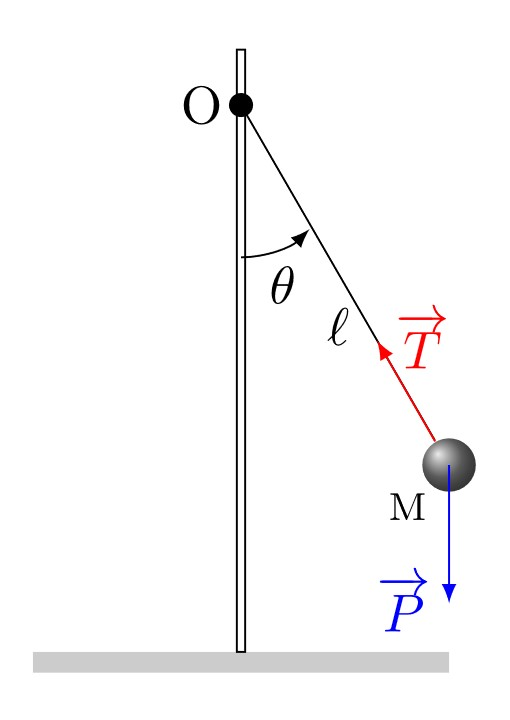
\includegraphics[width=5cm]{ch17pendule}
        % \captionof{figure}{Schéma du pendule simple.}
        % \label{fig:pendsimple}
    \end{center}
\end{minipage}

\section{Réaliser}

\begin{tror}{Important, hand}
    \bfseries
    Attention, la tige du pendule est en fibre de carbone et est TRES FRAGILE~;
    Ne pas serrer la vis de la masse trop fort sur la tige.
\end{tror}

\subsection{Réglages}

\begin{enumerate}
    \item Ouvrir le logiciel \texttt{Latispro}.
    \item Régler les paramètres d'acquisition~:
        
\includegraphics[width=0.05\textwidth]{bouton1} $200$ points de mesure~;
        choisir un temps total d'acquisition permettant d'avoir quelques
        oscillations visibles.
\end{enumerate}
\begin{enumerate}[resume, label=\sqenumi]
    \item Quelle doit alors être la fréquence
        d'échantillonnage de l'acquisition~?
\end{enumerate}
\begin{enumerate}[resume]
    \item Faire le zéro de l'oscillateur en appuyant sur le petit bouton à
        l'extrémité du fil noir près de la poulie, lorsque celui-ci est en
        position verticale.
\end{enumerate}

\subsection{Acquisition et enregistrement}

\begin{enumerate}
    \item Écarter le pendule d'un angle de $20\degres$ à $30\degres$ environ.
    \item Lancer l'acquisition~: 
\includegraphics[width=0.03\textwidth]{bouton2}
\end{enumerate}


\section{Valider}

\subsection{Exploitation de l'enregistrement}

\subsubsection{Visualisation des angles, vitesses et accélérations en fonction du temps}

\begin{enumerate}
    \item En utilisant la feuille de calcul, créer une nouvelle variable, notée
        \textit{angle}, correspondant à l'angle exprimé en radians.
    \item Visualiser \textit{angle} en fonction du temps~; ajuster l'échelle
        grâce au calibrage (en cliquant droit).
    \item Créer les variables \textit{deriv\_Pendule} (dérivée première) et
        \textit{dderiv\_Pendule} (dérivée seconde), en utilisant les fonctions
        traitements $\rightarrow$ calculs spécifiques $\rightarrow$ dérivée et
        dérivée seconde.
    \item À partir des variables \textit{deriv\_Pendule} et
        \textit{dderiv\_Pendule} (exprimées en degrés), introduire les variables
        \textit{deriv\_angle} et \textit{dderiv\_angle} exprimées en radians. 
    \item Afficher simultanément les trois courbes obtenues et les lisser en
        utilisant les fonctions traitements $\rightarrow$ calculs spécifiques
        $\rightarrow$ lissage.
\end{enumerate}
\begin{enumerate}[label=\sqenumi, start=4]
    \item Imprimer vos courbes.
    \item Déterminer et commenter les déphasages entre les différentes courbes.
        Justifier mathématiquement ces déphasages.
\end{enumerate}

\subsubsection{Propriété de l'énergie mécanique}

\begin{enumerate}[resume, label=\clenumi]
    \item Proposer une exploitation graphique permettant de visualiser
        graphiquement et simultanément la conservation de l'énergie mécanique
        ainsi que les échanges énergétiques entre énergie cinétique et énergie
        potentielle. Vous représenterez sur un même graphique $\Ec_p(t)$,
        $\Ec_c(t)$ et $\Ec_m(t)$.
\end{enumerate}
\begin{enumerate}[resume, label=\sqenumi]
    \item Imprimer les courbes et les commenter.
\end{enumerate}

\subsubsection{Approximation harmonique autour de la position d'équilibre}

\begin{enumerate}[resume, label=\clenumi]
    \item Proposer une exploitation permettant de vérifier la parabolisation
        (énergie potentielle est équivalente à un polynôme d'ordre 2 en $\tt$)
        de l'énergie potentielle autour de la position d'équilibre. Vous
        tracerez pour cela $\Ec_p(\tt)$.
\end{enumerate} \bigbreak
Vous pourrez ensuite faire une modélisation à partir d'un modèle parabolique
(pour une fois qu'on vous autorise à modéliser par autre chose qu'une droite…).
Vérifier visuellement que le modèle est compatible avec les données
expérimentales. \bigbreak
\begin{enumerate}[resume, label=\sqenumi]
    \item Imprimer et commenter. Faire le développement limité autour de $\tt=0$
        (position d'équilibre) de l'expression de l'énergie potentielle
        précédemment obtenue pour comparer. 
\end{enumerate}
 
\subsection{Amplitude et (non-)isochronisme des oscillations}

\subsubsection{Protocole expérimental}

\begin{enumerate}[resume, label=\sqenumi]
    \item Proposer puis réaliser un protocole expérimental qui permettrait de
        lever la contradiction historique présentée dans la partie S'approprier
        sans dépasser un angle initial de $60\degres$ environ (on pourra
        utiliser l'icône~: Outils $\rightarrow$ mesures automatiques).
    \item Présenter vos mesures sous forme d'un tableau $T\ind{exp} = f(\tt_0)$
        et d'une courbe expérimentale que vous imprimerez et commenterez.
        Conclure quant à l'isochronisme (ou non) des oscillations. 
    \item En déduire la valeur de $T\ind{iso}$ en tenant compte de vos
        différents mesurages \textbf{dans le cas où il y a isochronisme}.
\end{enumerate}

\subsubsection{Résolution numérique}

L'objectif de cette résolution numérique est de résoudre l'équation
différentielle non linéarisée et donc non analytique~: 
\[
    \tpp + {\w_0}^2 \sin(\tt) = 0
\]

\begin{enumerate}
    \item Dans un premier temps, vous allez compléter le script suivant sur
        \texttt{Capytale} à ce lien~:
        \url{https://capytale2.ac-paris.fr/web/c/eb53-1348043}. Il devra
        permettre de résoudre, pour une condition initiale $\tt_0$ donnée,
        l'équation différentielle ci-dessus à l'aide du schéma numérique python
        \texttt{solve\_ivp}. Pour ce faire, vous devrez importer
        \texttt{scipy.integrate} au début de votre script avec 

        \begin{python}
from scipy.integrate import solve_ivp
        \end{python}

        On prendra une période propre $T_0 = 1$ (par choix arbitraire).
        \bigbreak Pour vous aider, consulter la page suivante~:
        \url{https://tinyurl.com/pythonsolveivp}.
    \item Le script précédent sera ensuite amélioré afin de résoudre l'équation
        différentielle pour un ensemble de solutions initiales comprises entre
        $\tt_0 \approx 0$ et $\tt_0 = \pi/2$. Vous trouverez la fréquence de
        chaque solution grâce à une fonction \texttt{freqfinder} déjà créée
        l'occasion~; elle réalise la transformée de Fourier numérique de
        la solution temporelle (à l'aide de \texttt{numpy.fft}) afin d'en
        déduire le spectre puis la fréquence du pic spectral. Il vous faudra
        modifier la période propre par la valeur expérimentale $T\ind{iso}$. 
\end{enumerate}

\bigskip

\begin{enumerate}[label=\sqenumi, start=13]
    \item Expliquer sur \texttt{Capytale} (avec une cellule en
        \texttt{markdown}) en une dizaine de lignes les principales étapes de ce
        script.
    \item Construire, grâce à ce script, le graphe permettant d'obtenir la
        période $T\ind{simu}$ en fonction de l'amplitude initiale $\tt_0$. 
    \item Commenter l'influence des variables \texttt{duree} et
        \texttt{nb\_point\_temporel}. Faites des essais pour constater leur
        influence.
    \item Superposer à ce premier graphe vos résultats expérimentaux obtenus
        précédemment ($T\ind{exp} = f(\tt_0)$). Enregistrer votre travail sur
        \texttt{Capytale} et imprimer la courbe obtenue. 
    \item Les résultats numériques et expérimentaux sont-ils en accord~?
        Conclure.
\end{enumerate}

\end{document}
